\documentclass[11pt,a4paper]{article}
\usepackage{fontspec}
\usepackage{xcolor}
\usepackage{titlesec}
\usepackage{geometry}
\usepackage{cite}
\usepackage{float}
\usepackage{enumitem}
\usepackage{hyperref}
\usepackage{graphicx}
\usepackage{lmodern}
\renewcommand{\rmdefault}{lmss}

% Colors
\definecolor{primary}{RGB}{0,103,149}
\definecolor{secondary}{RGB}{128,179,211}

% Page geometry
\geometry{margin=2.5cm}

% Title formatting
\titleformat{\section}
  {\color{primary}\Large\bfseries}
  {\thesection}{1em}{}[\titlerule]
\titleformat{\subsection}
  {\color{primary}\large\bfseries}
  {\thesubsection}{1em}{}

% Hyperref setup
\hypersetup{
    colorlinks=true,
    linkcolor=primary,
    urlcolor=primary
}

\begin{document}

\title{\textcolor{primary}{\textbf{Free VPNs and Privacy: A Survey of Security Aware Users}}}
\author{Kurudunje Deekshith Shetty | Shitil Shetty}
\date{24th April, 2025}

\maketitle

\section{Introduction}

\textit{Disclaimer: This study is an extension to our main research project titled "Beyond the Price Tag: Examining User Behavior and Trust in Free VPN Services". Our research explores how much people trust free VPNs and whether they truly understand the privacy risks. This survey builds on
that by focusing on how security-aware user's perspective and how they evaluate free VPNs. The findings from this study will directly support and strengthen our main research. The references remain consistent with our main project.} \\

Virtual Private Networks (VPNs) are widely used to enhance online privacy and security. However, free VPN services often raise concerns about their business models, particularly regarding data privacy \cite{abbas2023,khan2018,ramesh2022}. This study surveys security-aware users to understand how their technical knowledge shapes their evaluation of free VPNs compared to non-technical users, their trust in these services, and the factors influencing their recommendations. Specifically, we address the following research questions: How do technically versed users evaluate free VPNs differently from general users? What technical and ethical concerns influence their trust? What role do transparency and auditing play in their trust levels? Would their knowledge impact VPN adoption recommendations? Are they more aware of the privacy implications of free VPNs? \cite{namara2020}

\section{Methods}

We conducted an online survey of 16 participants with varying levels of cybersecurity expertise, ranging from beginner to expert \cite{dutkowska2022}. Participants were asked about their VPN usage, technical knowledge, trust in free VPN providers, and concerns regarding data privacy. The survey included both closed-ended questions (Likert-scale ratings) and open-ended questions to capture detailed perspectives. Responses were analyzed to identify common themes and quantify concerns and trust levels.


\section{Results}

Participants demonstrated a high level of skepticism toward free VPNs, primarily due to concerns about data privacy and security. Most respondents (43.8\%) used a paid VPN, while 18.8\% used a free VPN, and 37.5\% did not use a VPN at all \cite{sombatruang2020}. Participants with greater VPN-specific knowledge (rated 4 or 5 on a 5-point scale) predominantly opted for paid VPNs, indicating a preference for services perceived as more secure. Surprisingly, those with higher general technical expertise (rated 4 or 5 on a 5-point scale) were more likely to use free VPNs or no VPN, suggesting that broad technical expertise may lead to diverse preferences, possibly due to confidence in mitigating risks independently.
\\\\
When evaluating free VPNs, participants emphasized technical and ethical concerns, distinguishing their perspectives from those of non-technical users. Many noted that non-technical users prioritize ease of use and cost, while security-aware users focus on protocols, encryption strength, and data logging policies. For example, one participant stated, ``I evaluate free VPNs by looking at their security protocols, data logging policies, and potential risks, while a non-technical user might focus mainly on ease of use and cost'' (cranky-wilbur). Another highlighted the business model, noting, ``I acknowledge that many free VPNs make money off of making you the product. If it's free, you're the product is my go-to'' (infallible-lalande).\\
The most prevalent concerns about free VPNs included data logging, weak encryption, potential malware, selling user data, and lack of transparency \cite{ikram2016,blancaflor2024}. Figure~\ref{Fig 1: Top Concerns About Free VPNs} illustrates the frequency of these concerns, with data logging and selling user data cited by nearly all respondents (15 and 16 out of 16, respectively). These concerns reflect a deep awareness of the privacy implications of free VPNs, with participants frequently mentioning the monetization of browsing history, IP addresses, and connection logs. One respondent noted, ``Free VPNs are most likely to monetize browsing history, connection logs, location data, and device information for advertising and analytics purposes'' (cranky-wilbur).

\begin{figure}[h]
    \centering
    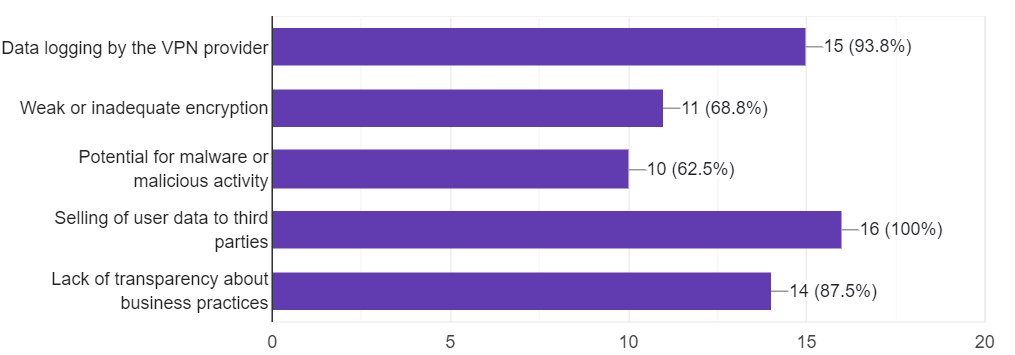
\includegraphics[width=1.0\textwidth]{fig 1.png} 
    \caption{Bar chart showing the frequency of concerns about free VPNs among respondents, with data logging and selling user data being the most cited.}
    \label{Fig 1: Top Concerns About Free VPNs}
\end{figure}


Trust in free VPN providers was notably low, with 37.5\% of respondents rating their trust at 1 (very low) and 37.5\% at 2 on a 5-point scale. Only 25\% rated their trust at 3 (neutral), and none rated higher. Table~\ref{Table 1: Trust in Free VPN Providers} summarizes the distribution of trust levels, highlighting the pervasive distrust among security-aware users. This distrust often stemmed from the perceived business model of free VPNs, with participants noting that data selling undermines privacy. One respondent remarked, ``They often collect and sell user data to make a profit, which defeats the purpose of privacy'' (cranky-wilbur).

\begin{table}[h] 
    \centering
    \renewcommand{\arraystretch}{1.5}
    \setlength{\tabcolsep}{12pt}
    \begin{tabular}{|l|c|r|}
        \hline
        Trust Level & Number of Respondents \\
        \hline 
        Trust Level 1   &  6   \\
        Trust Level 2   &  6   \\ 
        Trust Level 3   &  4   \\ 
        Trust Level 4   &  0   \\ 
        Trust Level 5   &  0   \\ 
        \hline
    \end{tabular}
    \caption{Table showing the distribution of trust levels in free VPN providers, with most respondents expressing very low trust.}
    \label{Table 1: Trust in Free VPN Providers}
\end{table}

Transparency and auditing were critical to increasing trust \cite{ramesh2023}. Respondents frequently cited public third-party audits, open-source codebases, transparent data handling policies, and jurisdictions outside surveillance alliances as trust-enhancing factors. For instance, one participant emphasized, ``Public third-party audits, Open-source codebase, Jurisdiction outside surveillance alliances, Transparent data handling policy'' (determined-mahavira). These factors suggest that verifiable assurances of privacy practices are essential for security-aware users.\\

The low trust in free VPNs translated into reluctance to recommend them, particularly to non-technical users as shown in Figure~\ref{Fig 2: Likely to Recommend}. Only 31.3\% of respondents were neutral about recommending free VPNs, while 68.7\% were unlikely or very unlikely to do so. This hesitancy reflects an understanding of the risks that non-technical users may not appreciate. One respondent noted, ``How easy it is to entrap people and give them a false sense of security where the reality could not be further from the truth'' (interesting-buck).

\begin{figure}[h]
    \centering
    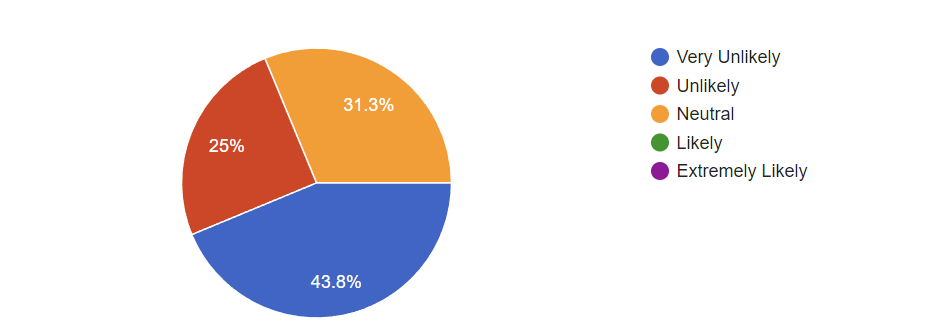
\includegraphics[width=1.0\textwidth]{fig 2.png} 
    \caption{Pie Chart showing how likely were the participants to recommend the usage of a free VPN.}
    \label{Fig 2: Likely to Recommend}
\end{figure}


\section{Discussion}

The findings confirm that security-aware users evaluate free VPNs with a critical lens, focusing on technical vulnerabilities and ethical concerns such as data monetization \cite{alshalan2016,mehrnezhad2022}. Unlike non-technical users, who may prioritize accessibility, these respondents emphasized encryption strength, logging policies, and transparency. Their low trust in free VPNs is driven by the perception that these services profit by selling user data, a concern supported by their identification of browsing history and connection logs as commonly monetized data types. \\

Transparency and independent auditing emerged as pivotal for building trust, suggesting that free VPN providers could improve perceptions by adopting open practices \cite{story2021}. The reluctance to recommend free VPNs to non-technical users underscores a protective stance, driven by awareness of privacy risks that less knowledgeable users might overlook. This aligns with the broader theme of heightened privacy awareness among technically versed users, who view free VPNs as inherently risky due to their business models.


\section{Conclusions and Future Directions}

This survey highlights the skepticism of security-aware users toward free VPNs, driven by concerns about data privacy, weak security, and lack of transparency. These users differ significantly from non-technical users in their focus on technical and ethical risks, and their knowledge reduces their willingness to recommend free VPNs. Transparency and auditing are critical to fostering trust, but the prevailing view that ''if it's free, you're the product'' remains a significant barrier. \\

Future research could explore the perspectives of non-technical users to directly compare their evaluations with those of technical users \cite{moore2024}. Additionally, investigating the actual data practices of free VPN providers through technical audits could validate or challenge user perceptions \cite{fassl2023}. Examining the impact of educational interventions on non-technical users’ VPN choices could inform strategies to bridge the knowledge gap identified in this study.

\bibliographystyle{plain}
\bibliography{references}


\end{document}